\documentclass[11pt]{aghdpl}
% \documentclass[en,11pt]{aghdpl}  % praca w języku angielskim

% Lista wszystkich języków stanowiących języki pozycji bibliograficznych użytych w pracy.
% (Zgodnie z zasadami tworzenia bibliografii każda pozycja powinna zostać utworzona zgodnie z zasadami języka, w którym dana publikacja została napisana.)
\usepackage[english,polish]{babel}

% Użyj polskiego łamania wyrazów (zamiast domyślnego angielskiego).
\usepackage{polski}

\usepackage[utf8]{inputenc}

% dodatkowe pakiety

\usepackage{mathtools}
\usepackage{amsfonts}
\usepackage{amsmath}
\usepackage{amsthm}
\usepackage{graphicx}
\usepackage{wrapfig}
\usepackage{gensymb}

% --- < bibliografia > ---

\usepackage[
style=numeric,
sorting=none,
%
% Zastosuj styl wpisu bibliograficznego właściwy językowi publikacji.
language=autobib,
autolang=other,
% Zapisuj datę dostępu do strony WWW w formacie RRRR-MM-DD.
urldate=iso8601,
% Nie dodawaj numerów stron, na których występuje cytowanie.
backref=false,
% Podawaj ISBN.
isbn=true,
% Nie podawaj URL-i, o ile nie jest to konieczne.
url=false,
%
% Ustawienia związane z polskimi normami dla bibliografii.
maxbibnames=3,
% Jeżeli używamy BibTeXa:
backend=bibtex
]{biblatex}

\usepackage{csquotes}
% Ponieważ `csquotes` nie posiada polskiego stylu, można skorzystać z mocno zbliżonego stylu chorwackiego.
\DeclareQuoteAlias{croatian}{polish}

\addbibresource{bibliografia.bib}

% Nie wyświetlaj wybranych pól.
%\AtEveryBibitem{\clearfield{note}}


% ------------------------
% --- < listingi > ---

% Użyj czcionki kroju Courier.
\usepackage{courier}

\usepackage{listings}
\lstloadlanguages{TeX}

\lstset{
	literate={ą}{{\k{a}}}1
           {ć}{{\'c}}1
           {ę}{{\k{e}}}1
           {ó}{{\'o}}1
           {ń}{{\'n}}1
           {ł}{{\l{}}}1
           {ś}{{\'s}}1
           {ź}{{\'z}}1
           {ż}{{\.z}}1
           {Ą}{{\k{A}}}1
           {Ć}{{\'C}}1
           {Ę}{{\k{E}}}1
           {Ó}{{\'O}}1
           {Ń}{{\'N}}1
           {Ł}{{\L{}}}1
           {Ś}{{\'S}}1
           {Ź}{{\'Z}}1
           {Ż}{{\.Z}}1,
	basicstyle=\footnotesize\ttfamily,
}

% ------------------------

\AtBeginDocument{
	\renewcommand{\tablename}{Tabela}
	\renewcommand{\figurename}{Rys.}
}

% ------------------------
% --- < tabele > ---

\usepackage{array}
\usepackage{tabularx}
\usepackage{multirow}
\usepackage{booktabs}
\usepackage{makecell}
\usepackage[flushleft]{threeparttable}

% defines the X column to use m (\parbox[c]) instead of p (`parbox[t]`)
\newcolumntype{C}[1]{>{\hsize=#1\hsize\centering\arraybackslash}X}


%---------------------------------------------------------------------------

\author{Marek Jachym, Wojciech Konieczkowicz}
\shortauthor{M. Jachym~~W. Konieczkowicz}

%\titlePL{Przygotowanie bardzo długiej i pasjonującej pracy dyplomowej w~systemie~\LaTeX}
%\titleEN{Preparation of a very long and fascinating bachelor or master thesis in \LaTeX}

\titlePL{Symulacja zagrożenia lawinowego w~Tatrach Polskich}
\titleEN{}


\shorttitlePL{Symulacja zagrożenia lawinowego w~Tatrach Polskich} % skrócona wersja tytułu jeśli jest bardzo długi
\shorttitleEN{Preparation of a long and fascinating thesis in \LaTeX}

\thesistype{Symulacja Dyskretna Systemów Złożonych}
%\thesistype{Master of Science Thesis}

\supervisor{dr hab. inż. Jarosław Wąs}
%\supervisor{Marcin Szpyrka PhD, DSc}

\degreeprogramme{Informatyka}
%\degreeprogramme{Computer Science}

\date{2020}

\department{}
%\department{Department of Applied Computer Science}

\faculty{Wydział Elektrotechniki, Automatyki,\protect\\[-1mm] Informatyki i Inżynierii Biomedycznej}
%\faculty{Faculty of Electrical Engineering, Automatics, Computer Science and Biomedical Engineering}

\acknowledgements{Serdecznie dziękuję \dots tu ciąg dalszych podziękowań np. dla promotora, żony, sąsiada itp.}


\setlength{\cftsecnumwidth}{10mm}

%---------------------------------------------------------------------------
\setcounter{secnumdepth}{4}
\brokenpenalty=10000\relax

\begin{document}

\titlepages

% Ponowne zdefiniowanie stylu `plain`, aby usunąć numer strony z pierwszej strony spisu treści i poszczególnych rozdziałów.
\fancypagestyle{plain}
{
	% Usuń nagłówek i stopkę
	\fancyhf{}
	% Usuń linie.
	\renewcommand{\headrulewidth}{0pt}
	\renewcommand{\footrulewidth}{0pt}
}

\setcounter{tocdepth}{2}
\tableofcontents
\clearpage

%\chapter{Wprowadzenie}
\label{cha:wprowadzenie}

\section{Cel}
Celem niniejszej pracy jest stworzenie symulacji, która dostarcza w czasie rzeczywistym informacji dotyczących możliwego zagrożenia lawinowego na terenie Tatr w Polsce. 

%---------------------------------------------------------------------------

\section{Opis problemu}

Lawiny śnieżne są powszechnie występującym zagrożeniem na całym świecie i stanowią niebezpieczeństwo zarówno dla ludzi, jak i~biznesu oraz infrastruktury. Instytucje w różnych państwach alarmują o zagrożeniu lawinowym w podobny sposób, choć można zauważyć, że im większe zagrożenie stanowi zjawisko samoistnego ruchu śniegu, tym bardziej szczegółowe są prognozy. 

Głównym problemem przy określaniu ryzyka lawinowego jest złożoność tego zjawiska. Zależy ono zarówno od czynników stałych, do których zalicza się np. ukształtowanie terenu (1. typ uwarunkowań) oraz zmiennych, dotyczących stanu śniegu (2. typ uwarunkowań) oraz warunków meteorologicznych (3. typ uwarunkowań) (Woszczek 2016). Polskie instytucje wydają regularnie tzw. komunikaty lawinowe, są one jednak jedynie ogólnym zapisem zagrożenia - ratownicy zastrzegają, że informacje zawarte w komunikacie stanowią tylko podstawę do samodzielnej oceny. 

Przedmiotem poniższej pracy jest więc próba zastosowania technologii, by zapewnić system wspomagający decyzje ekspertów w celu tworzenia jeszcze bardziej precyzyjnych ostrzeżeń. Symulacja sama w sobie nie stanowi profesjonalnego narzędzia, ale zawiera koncepcje i rozwiązania, które można zastosować przy tworzeniu niezawodnego i złożonego narzędzia dla państwowych instytucji. 

\section{Możliwe rozwiązanie}
Na świecie modele przewidujące zagrożenie są tworzone w oparciu o metody statystyczne oraz metody uczenia maszynowego takie jak analiza najbliższego sąsiedztwa (ang. nearest neighbor analysis), analiza skupień (ang. cluster analysis), czy drzewa klasyfikacyjne (ang. classification trees) (Joshi, Kumar, Srivastava, Sachdeva, Ganju 2018). Są to jednak rozwiązania stworzone na podstawie wieloletnich pomiarów (również dotyczących warunków pokrywy śnieżnej), do których nie uzyskano dostępu. Zdecydowano się więc oprzeć na wnioskach autorów publikacji, charakteryzujących najważniejsze czynniki stwarzające ryzyko. 
 
W celu jak najdokładniejszego określania ryzyka wykorzystano bardzo precyzyjne informacje dotyczące ukształtowania terenu oraz dane pogodowe (dane dotyczące śniegu nie są ogólnodostępne i ich zmierzenie wymaga specjalistycznej wiedzy oraz narzędzi). 

Korzystając z danych topograficznych uproszczono ukształtowanie powierzchni Tatr (każdy z obszarów  o powierzchni ponad 2 km$^2$ reprezentowany jest przy pomocy około 110 punktów) i obliczono odpowiednie cechy. Następnie w połączeniu z cechami dotyczącymi warunków atmosferycznych możliwe stało się określenie ryzyka dla każdego takiego obszaru przy pomocy stworzonego wcześniej drzewa decyzyjnego. Dzięki takiemu podejściu, cały obszar Tatr Polskich podlega obserwacji, a w razie wystąpienia sprzyjających warunków (wykorzystano 2 z 3 istniejących uwarunkowań) w sposób zautomatyzowany wydaje się odpowiednie ostrzeżenia.

%---------------------------------------------------------------------------


W rodziale~\ref{cha:pierwszyDokument} przedstawiono podstawowe informacje dotyczące struktury dokumentów w \LaTeX u. Alvis~\cite{Alvis2011} jest językiem 



















\chapter{Wprowadzenie}
\label{cha:wprowadzenie}

\section{Cel}
Celem niniejszej pracy jest stworzenie symulacji, która dostarcza w czasie rzeczywistym informacji dotyczących możliwego zagrożenia lawinowego na terenie Tatr w Polsce. 

%---------------------------------------------------------------------------

\section{Opis problemu}

Lawiny śnieżne są powszechnie występującym zagrożeniem na całym świecie i stanowią niebezpieczeństwo zarówno dla ludzi, jak i~biznesu oraz infrastruktury. Instytucje w różnych państwach alarmują o zagrożeniu lawinowym w podobny sposób, choć można zauważyć, że im większe zagrożenie stanowi zjawisko samoistnego ruchu śniegu, tym bardziej szczegółowe są prognozy. 

Głównym problemem przy określaniu ryzyka lawinowego jest złożoność tego zjawiska. Zależy ono zarówno od czynników stałych, do których zalicza się np. ukształtowanie terenu (1. typ uwarunkowań) oraz zmiennych, dotyczących stanu śniegu (2. typ uwarunkowań) oraz warunków meteorologicznych (3. typ uwarunkowań) (Woszczek 2016). Polskie instytucje wydają regularnie tzw. komunikaty lawinowe, są one jednak jedynie ogólnym zapisem zagrożenia - ratownicy zastrzegają, że informacje zawarte w komunikacie stanowią tylko podstawę do samodzielnej oceny. 

Przedmiotem poniższej pracy jest więc próba zastosowania technologii, by zapewnić system wspomagający decyzje ekspertów w celu tworzenia jeszcze bardziej precyzyjnych ostrzeżeń. Symulacja sama w sobie nie stanowi profesjonalnego narzędzia, ale zawiera koncepcje i rozwiązania, które można zastosować przy tworzeniu niezawodnego i złożonego narzędzia dla państwowych instytucji. 

\section{Możliwe rozwiązanie}
Na świecie modele przewidujące zagrożenie są tworzone w oparciu o metody statystyczne oraz metody uczenia maszynowego takie jak analiza najbliższego sąsiedztwa (ang. nearest neighbor analysis), analiza skupień (ang. cluster analysis), czy drzewa klasyfikacyjne (ang. classification trees) (Joshi, Kumar, Srivastava, Sachdeva, Ganju 2018). Są to jednak rozwiązania stworzone na podstawie wieloletnich pomiarów (również dotyczących warunków pokrywy śnieżnej), do których nie uzyskano dostępu. Zdecydowano się więc oprzeć na wnioskach autorów publikacji, charakteryzujących najważniejsze czynniki stwarzające ryzyko. 
 
W celu jak najdokładniejszego określania ryzyka wykorzystano bardzo precyzyjne informacje dotyczące ukształtowania terenu oraz dane pogodowe (dane dotyczące śniegu nie są ogólnodostępne i ich zmierzenie wymaga specjalistycznej wiedzy oraz narzędzi). 

Korzystając z danych topograficznych uproszczono ukształtowanie powierzchni Tatr (każdy z obszarów  o powierzchni około 4 km$^2$ reprezentowany jest przy pomocy około 110 punktów) i obliczono odpowiednie cechy. Następnie w połączeniu z cechami dotyczącymi warunków atmosferycznych możliwe stało się określenie ryzyka dla każdego takiego obszaru przy pomocy stworzonego wcześniej drzewa decyzyjnego. Dzięki takiemu podejściu, cały obszar Tatr Polskich podlega obserwacji, a w razie wystąpienia sprzyjających warunków (wykorzystano 2 z 3 istniejących uwarunkowań) w sposób zautomatyzowany wydaje się odpowiednie ostrzeżenia.

%---------------------------------------------------------------------------



















\chapter{Przykłady elementów pracy dyplomowej}

\section{Liczba}

Pakiet \texttt{siunitx} zadba o to, by liczba została poprawnie sformatowana: \\
\begin{center}
	\num{1234567890.0987654321}
\end{center}


\section{Rysunek}

Pakiet \texttt{subcaption} pozwala na umieszczanie w podpisie rysunku odnośników do ,,podilustracji'': \\

\begin{figure}[h]
	\centering
	\begin{subfigure}{0.35\textwidth}
		\centering
		\framebox[2.0\width]{A}
		\subcaption{\label{subfigure_a}}
	\end{subfigure}
	\begin{subfigure}{0.35\textwidth}
		\centering
		\framebox[2.0\width]{B}
		\subcaption{\label{subfigure_b}}
	\end{subfigure}
	
	\caption{\label{fig:subcaption_example}Przykład użycia \texttt{\textbackslash subcaption}: \protect\subref{subfigure_a} litera A, \protect\subref{subfigure_b} litera B.}
\end{figure}

\section{Tabela}

Pakiet \texttt{threeparttable} umożliwia dodanie do tabeli adnotacji: \\

\begin{table}[h]
	\centering
	
	\begin{threeparttable}
		\caption{Przykład tabeli}
		\label{tab:table_example}
		
		\begin{tabularx}{0.6\textwidth}{C{1}}
			\toprule
			\thead{Nagłówek\tnote{a}} \\
			\midrule
			Tekst 1 \\
			Tekst 2 \\
			\bottomrule
		\end{tabularx}
		
		\begin{tablenotes}
			\footnotesize
			\item[a] Jakiś komentarz\textellipsis
		\end{tablenotes}
		
	\end{threeparttable}
\end{table}

\section{Wzory matematyczne}

Czasem zachodzi potrzeba wytłumaczenia znaczenia symboli użytych w równaniu. Można to zrobić z użyciem zdefiniowanego na potrzeby niniejszej klasy środowiska \texttt{eqwhere}.

\begin{equation}
E = mc^2
\end{equation}
gdzie
\begin{eqwhere}[2cm]
	\item[$m$] masa
	\item[$c$] prędkość światła w próżni
\end{eqwhere}

Odległość półpauzy od lewego marginesu należy dobrać pod kątem najdłuższego symbolu (bądź listy symboli) poprzez odpowiednie ustawienie parametru tego środowiska (domyślnie: 2 cm).

\chapter{Symulacja zjawiska - implementacja i szczegóły techniczne}

\section{Wybór języka programowania}

Językiem który postanowiliśmy wybrać do implementacji symulacji przedstawionego powyżej problemu wybrano język Python w wersji \textbf{3.7.x}.

Ze względu na jego prostotę, wydajność i obszerny wybór bibliotek zewnętrznych wybraliśmy zamiast innych, również bardzo wydajnych ale bardziej skomplikowanych języków takich jak C++ czy Java.

% \clearpage

\section{Narzędzia wykorzystywane w trakcie tworzenia projektu}
\begingroup
\subsection{Środowisko programowania}
\begin{wrapfigure}{L}{0.55\textwidth}

	\centering
	
\includegraphics[width=0.25\textwidth]{PyCharm_Logo.png}
	\caption{\label{fig:frog2}PyCharm Community}

\end{wrapfigure}

Wykorzystano \textbf{PyCharm Community 2019.3}, rozbudowane, potężne i wyposażone w dużą ilość dodatkowych narzędzi środowisko stworzone do pracy z językiem Python. Dostępne jest w dwóch wersjach, Professional oraz Community będąca wersją open-source przez co idealnie nadała się do wykorzystania przy naszym projekcie.

\endgroup
\clearpage

\subsection{Wybrane biblioteki zewnętrzne języka Python}
Jak wspomniano wcześniej, Python jest bardzo popularnym językiem przez co posiada wiele bibliotek zewnętrznych.

Do implementacji symulacji problemu wykorzystano następujące biblioteki zewnętrzne:

\begin{enumerate}
	\item \textbf{PyQt5} - oferująca zestaw narzędzi do budowy graficznego interfejsu użytkownika
	\item \textbf{pyowm} - oferująca zestaw narzędzi do eksploatacji API Open Weather Map
	\item \textbf{laspy} - zestaw funkcji umożliwiająca wykonywanie wielu operacji na plikach .las
	\item \textbf{paramiko} - moduł umożliwiający komunikację SSH z poziomu skryptu w Pythonie
	\item \textbf{pyvista} - biblioteka zawierająca implementację algorytmu triangulacji Delaunaya
\end{enumerate}

\subsection{Usługi chmurowe Google Cloud Platform i dane pogodowe}
\begingroup
\begin{wrapfigure}{L}{0.45\textwidth}
	
	\centering
	
\includegraphics[width=0.25\textwidth]{gcp_logo.png}
	
\end{wrapfigure}
Kluczowym, z punktu widzenia projektu, okazało się znalezienie rozwiązania problemu ciągłej aktualizacji danych pogodowych. Z powodu iż dane muszą być nieustannie aktualizowane co 8 godzin, jedna z maszyn roboczych autorów musiałaby pracować bez przerwy. Nie jest to w żadnym stopniu rozwiązanie optymalne. Zdecydowano się na skorzystanie z darmowego okresu próbnego oferowanego na platformie \textbf{Google Cloud Platform}. Oferta Google zawarła w sobie możliwość stworzenia instancji maszyny wirtualnej operującej na systemie \textbf{Debian 10 Buster} co otworzyło drogę do rozwiązania problemu ciągłej aktualizacji danych pogodowych.
\clearpage

Dane pogodowe pobierane są co 8 godzin, o godzinach 00:00, 08:00 i 16:00 przy pomocy skryptu \textbf{weather\_conditions.py} który korzysta z biblioteki \textbf{pyowm}
\begin{lstlisting}[language=Python]
 weather_conditions.py
 
 #!/usr/bin/python2.7
 import pyowm
 import os
 import time
 import tarfile
 #ZMIENNA path REPREZENTUJE ODPOWIEDNIE ŚCIEŻKI DO PLIKÓW
 def get_weather_conditions(map_name):
 # UTWÓRZ ODPOWIEDNI FOLDER JEŻELI NIE ISTNIEJE
 if os.path.isdir(path):
 	pass
 else:
 	path = path
 os.mkdir(path)
 # WSPÓŁRZĘDNE ODPOWIEDNIEGO OBSZARU I CZAS POBRANIA DANYCH
 coords = extract_coords(map_name)
 czas_pomiaru = str(time.ctime()).split(" ")
 # POBRANIE DANYCH POGODOWYCH
 owm = pyowm.OWM("7202a85833f71127c0a0b4fefc86ea2a")
 observation = owm.weather_around_coords(float(coords["N_lat"]), float(coords["W_long"]))
 
 # USUWANIE NAJSTARSZEGO POMIARU I ZASTĄPIENIE GO NOWYM
 data = os.listdir(path)
 data.sort()
 if len(data) >= 6:
 	os.remove(path)
 # STWÓRZ PLIK ZAWIERAJĄCY AKTUALNE DANE POGODOWE
 filename = str(observation[0].get_weather().get_reference_time('date'))[0:10]
 data = open(path, "w+")
 data.write(str(observation[0].get_weather().get_temperature('celsius')['temp']) + "\n")
 data.write(str(observation[0].get_weather().get_snow()) + "\n")
 data.write(str(observation[0].get_weather().get_wind('meters_sec')) + "\n")
 data.write(str(observation[0].get_weather().get_rain()) + "\n")

\end{lstlisting}
\clearpage
\subsubsection{Harmonogram pobrania danych}
Za odpowiedni czas pobrania danych odpowiada narzędzie uniksopodobnych systemów operacyjnych \textbf{cron}. Jest to realizowane za pomocą odpowietnich wpisów w pliku \textbf{crontab}
\begin{verbatim}
	0 6 * * * /usr/bin/python /home/marekjachym99/lavalanche/weather_conditions.py

	0 14 * * * /usr/bin/python /home/marekjachym99/lavalanche/weather_conditions.py
	
	0 22 * * * /usr/bin/python /home/marekjachym99/lavalanche/weather_conditions.py	
\end{verbatim}



\chapter{Graficzny interfejs użytkownika}
Do stworzenia GUI (ang. Graphical User Interface) wykorzystano wcześniej wspomnianą bibliotekę PyQT5 oferującą zestaw narzędzi do budowy interfejsu użytkownika z użyciem klas QT
\section{Pierwszy etap implementacji}
Czytelny, prosty i przejrzysty interfejs użytkownika jest podstawą każdej dobrej aplikacji, niestety ze względu na wyzwania jakie niosła za sobą synchronizacja posiadanych map reprezentowanych przez zbiór plików .las z mapą geograficzną np. z Google Maps, nanoszenie zagrożeń na interaktywną mapę okazało się chwilowo poza zasięgiem.
\subsection{Mapa Tatr}
\begingroup
\begin{figure}[h]
	\centering
	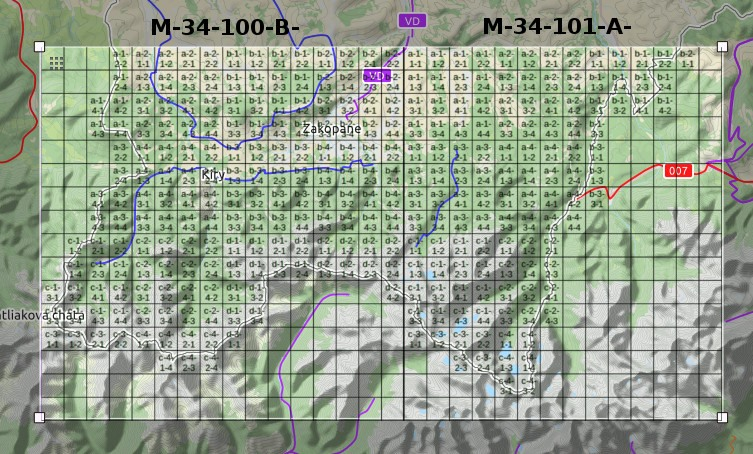
\includegraphics[scale=0.4]{tlo.png}
	\caption{Oryginalna mapa}
\end{figure}
\endgroup
\section{Etap drugi - główne okno aplikacji}
Stwierdzono, że główne okno aplikacji powinno zawierać jak najmniej zbędnych elementów i być czytelne jak i przykuwające uwagę, z tego powodu na ekranie głównym aplikacji widnieje piękny widok na Morskie Oko wraz z okalającymi je szczytami widziane ze schroniska.
\begingroup
\begin{figure}[h]
	\centering
	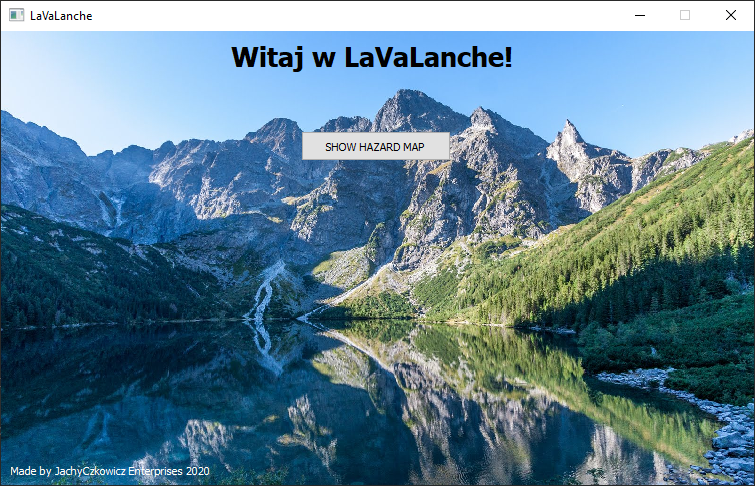
\includegraphics[scale=0.6]{main_window.png}
	\caption{Okno główne aplikacji \\ źródło: http://podrozniczeretrospekcje.blogspot.com}
\end{figure}
\endgroup
\clearpage
\section{Etap trzeci - interaktywna mapa Tatr}
Wykorzystując otrzymaną wcześniej mapę Tatr, postanowiono nałożyć na poszczególne kwadraty przyciski z których każdy odnosi się do zawartego pod nim obszaru. 

\begingroup
\begin{figure}[h]
	\centering
	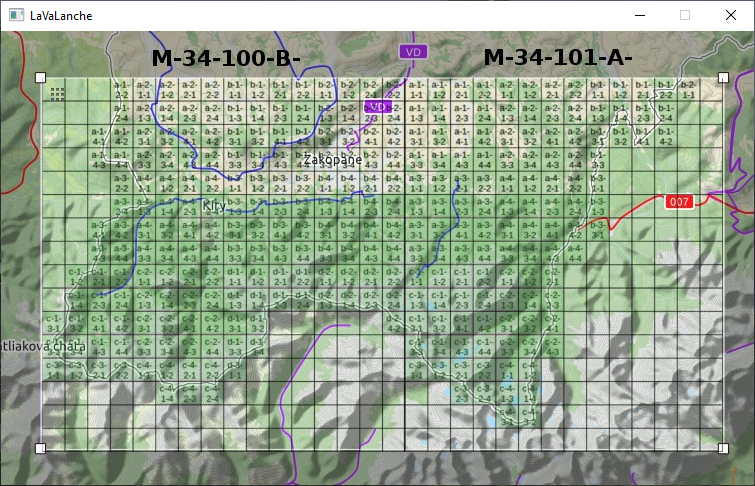
\includegraphics[scale=0.6]{map_window.png}
	\caption{Mapa z naniesionymi na nią przyciskami}
\end{figure}
\endgroup

Założono, że zagrożenie lawiną obliczane będzie tylko dla obszarów znajdujących się na południe od Zakopanego z tego względu iż ukształtowanie terenu na północ od tego miejsca praktycznie wyklucza wystąpienie jakiejkolwiek lawiny i nie ma tam historii występowania lawin, dlatego przyciski, które kolorowane są według poniższej legendy, znajdują się tylko na mniej więcej połowie obszarów. 
\begingroup
\begin{figure}[h]
	\centering
	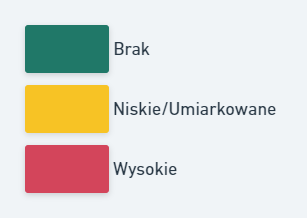
\includegraphics[scale=0.6]{kolorowanie.png}
	\caption{Legenda kolorów przycisków}
\end{figure}
\endgroup


\clearpage
\section{Etap czwarty - okna detaliczne}
Ostatni, lecz nie mniej ważny niż pozostałe etap, zakładał implementację okien detalicznych dla każdego obszaru autonomicznego tj. obszaru reprezentowanego przez jeden plik .las. W oknie detalicznym znajdują się takie dane jak:
\begin{enumerate}[label=-]
	\item Stopień ryzyka
	\item Charakterystyczne obiekty na danym terenie np. szczyty
	\item Cechy zwiększające zagrożenie
\end{enumerate}

\begingroup
\begin{figure}[h]
	\centering
	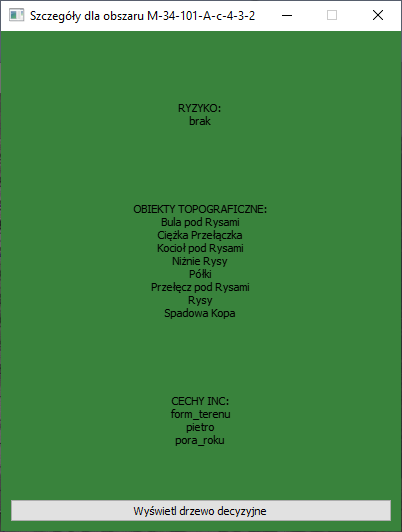
\includegraphics[scale=0.6]{detail_window.png}
	\caption{Okienko detaliczne}
\end{figure}
\endgroup
\clearpage
\section{Obsługa aplikacji i jej działanie}
Przed każdym uruchomieniem aplikacji aktualizowane są dane pogodowe z całego obszaru Tatr po polskiej stronie. Następnie ukazuje się okno główne aplikacji.

Na samym środku widnieje przycisk ''SHOW HAZARD MAP'' który po przyciśnięciu wyłącza okno główne i przechodzi do okna z interaktywną mapą obszaru.

W oknie interaktywnej mapy widnieją przyciski o kolorze odpowiadającym stopniowi zagrożnienia, każdy z przycisków włącza okno detaliczne dla odpowiedniego obszaru autonomicznego. Na chwilę obecną nie ma możliwości powrotu do ekranu głównego.












% itd.
% \appendix
% \include{dodatekA}
% \include{dodatekB}
% itd.

\printbibliography

\end{document}
